\documentclass[9pt,mathserif]{beamer}
%\documentclass[11pt,mathserif,aspectratio=1610]{beamer}
\usepackage{amsmath}
\usepackage{mathtools}
\usepackage{tikz} 
\usepackage{media9}
\usepackage{algorithm} % must read after hyperref
\usepackage{algorithmic}
\usepackage{subfigure,MnSymbol,pdfpages}
\usepackage{graphicx,color,colortbl}
\usepackage{bm,amsfonts,graphics}
\usepackage[export]{adjustbox}
\setbeamercolor{block title}{bg=blue!55,fg=black}%bg=background, fg= foreground
\setbeamercolor{block body}{bg=blue!20,fg=black}%bg=background, fg= foreground

\usepackage{amsmath}
\usepackage{mathtools}
\usepackage{tikz}
%\usepackage{movie15}
\usepackage{algorithm} % must read after hyperref
\usepackage{algorithmic}
\usepackage{subfigure,MnSymbol}
\usepackage{graphicx,color,colortbl}
%\usepackage[footnotesize,bf]{caption}
\usepackage{bm,amsfonts,graphics}
\usepackage{tikz,tkz-graph,tkz-arith,tkz-berge}
\usetikzlibrary{arrows,shapes,positioning}

\graphicspath{{./}{figures/}}
\usepackage{multicol}

\newtheorem{thm}{Theorem}
\newtheorem{lem}{Lemma}
\newtheorem{prop}{Proposition}
\newtheorem{rem}{Remark}

\newcommand{\jcols}[4]{
\begin{columns}[T]\begin{column}[T]{#3\textwidth} #1 \end{column}
\begin{column}[T]{#4\textwidth} #2 \end{column}
\end{columns}}

\newcommand{\jcolsb}[4]
{\begin{columns}[b]
\begin{column}{#3\textwidth} #1 \vspace{0pt}
\end{column}
\begin{column}{#4\textwidth} #2 \vspace{0pt}
\end{column}
\end{columns}}

\newcommand{\jcolsc}[4]
{\begin{columns}[c]
\begin{column}{#3\textwidth} #1 \vspace{0pt}
\end{column}
\begin{column}{#4\textwidth} #2 \vspace{0pt}
\end{column}
\end{columns}}
\mode<presentation>
{
	\usetheme{ACL}
        \setbeamercovered{transparent=0}
}

\makeatletter
\newdimen\labelwidthi
\newdimen\labelwidthii
\newdimen\labelwidthiii
\newdimen\labelwidthiv
\def\normal@labelsep{0.2em}
\labelsep\normal@labelsep
\settowidth{\labelwidthi}{iii}
\settowidth{\labelwidthii}{ii}
\settowidth{\labelwidthiii}{iii}
%\settowidth{\labelwidthiv}{i}
\setlength\leftmargini{0pt}
\setlength\leftmarginii{1.5ex}
\setlength\leftmarginiii{1.5ex}

\leftmargini\labelwidthi    \advance\leftmargini\labelsep
\leftmarginii\labelwidthii  \advance\leftmarginii\labelsep
\leftmarginii\labelwidthiii \advance\leftmarginiii\labelsep

%\leftmarginii\labelwidthiv  \advance\leftmarginiv\labelsep
%\def\setleftmargin#1#2{\settowidth{\@tempdima}{#2}\labelsep\normal@labelsep
%  \csname labelwidth#1\endcsname\@tempdima
%  \@tempdimb\@tempdima \advance\@tempdimb\labelsep
%  \csname leftmargin#1\endcsname\@tempdimb}
%\def\@listI{\leftmargin\leftmargini
%  \labelwidth\labelwidthi \labelsep\normal@labelsep
%  \topsep \z@ \partopsep\z@ \parsep\z@ \itemsep\z@
%  \listparindent 1em}
%\def\@listii{\leftmargin\leftmarginii
%  \labelwidth\labelwidthii \labelsep\normal@labelsep
%  \topsep\z@ \partopsep\z@ \parsep\z@ \itemsep\z@
%  \listparindent 1em}
%\def\@listiii{\leftmargin\leftmarginiii
%  \labelwidth\labelwidthiii \labelsep\normal@labelsep
%  \topsep\z@ \partopsep\z@ \parsep\z@ \itemsep\z@
%  \listparindent 1em}
%\def\@listiv{\leftmargin\leftmarginiv
%  \labelwidth\labelwidthiv \labelsep\normal@labelsep
%  \topsep\z@ \partopsep\z@ \parsep\z@ \itemsep\z@
%  \listparindent 1em}
%\let\@listi\@listI
%\@listi
\makeatother

\logo{

\includegraphics[height = 0.6cm,trim=0 50 0 0,clip]{AO-logo-high_color-top-MIT}

\includegraphics[height = 0.5cm,trim=0 0 0 0,clip]{ACL_logo}
}

\setbeamerfont{frametitle}{size=\large,series=\bfseries}
%\setbeamertemplate{frametitle}[default][center]
\setbeamerfont{title}{size=\large,series=\bfseries}
\setbeamerfont{framesubtitle}{series=\mdseries,size=\large}
\graphicspath{{./}{figures/}}
\usepackage[square, numbers, comma]{natbib}	% use Natbib for author-name
									% citations. In a presentation,
									% this is more legible than pure
									% numbers, like [21]. Google
									% "natbib" for more information.
									% Instead of "\cite{abc}", use
									% "\citep{abc}" or "\citet{abc}"
\bibliographystyle{plainnat}		% Natbib specific
%\bibpunct{(}{)}{,}{a}{}{,}			% Natbib specific

\definecolor{Maroon}{RGB}{112,0,0}
\definecolor{Crimson}{RGB}{200,0,0}
\definecolor{purple}{RGB}{112,0,112}

\newcommand{\bee}{\begin{enumerate}}
\newcommand{\eee}{\end{enumerate}}
\newcommand{\bi}{\begin{itemize}}
\newcommand{\bii}{\begin{itemize}\small}
\newcommand{\beee}{\begin{enumerate}\scriptsize}
\newcommand{\biii}{\begin{itemize}\footnotesize}
\newcommand{\ei}{\end{itemize}}
\newcommand{\jtem}{\vfill\item}
\newcommand{\bea}{\begin{eqnarray}}
\newcommand{\eea}{\end{eqnarray}}
\newcommand{\argmax}{\operatornamewithlimits{argmax}}
\newcommand{\njra}{\color{red} $\Rightarrow$~\color{black}}
\newcommand{\nred}[1]{{\tiny \color{red} XX #1 XX\color{black}}}
%\newcommand{\jframe}[1]{\begin{frame}\nred{#1}\end{frame}}
\newcommand{\jframe}[2]{\begin{frame}\frametitle{#1} #2 \end{frame}}
\newcommand{\jframeb}[2]{\begin{frame}[t]{#1} \begin{itemize} #2 \end{itemize} \end{frame}}
\newcommand{\jframet}[2]{\begin{frame}[t]\frametitle{#1} #2 \end{frame}}
\newcommand{\ji}[2]{\begin{itemize}\setlength{\itemsep}{#1mm}{#2}\end{itemize}}
\newcommand{\jen}[2]{\begin{enumerate}\setlength{\itemsep}{#1mm}{#2}\end{enumerate}}
\newcommand{\bc}{\begin{center}}
\newcommand{\ec}{\end{center}}
\newcommand{\todo}[1]{{\color{magenta} XX- #1 -XX}}
\newcommand{\XX}[1]{{\color{red} XX- #1 -XX}}
\newcommand{\alertr}[1]{\textbf{\color{red} #1}}

\setbeamercovered{transparent=10}
\setbeamercolor{title}{bg = black!10}
\setbeamercolor{frametitle}{bg = black!0}
\setbeamercolor{thm}{bg = black!0}
%\setbeamercolor{alerted text}{fg=blue}
%\setbeamerfont{alerted text}{series = \bfseries}

%{use = palette secondary, bg = palette secondary.bg}

\setbeamercolor{normal text}{fg=black}  
\setbeamertemplate{enumerate items}[ball]
\setbeamertemplate{enumerate subitem}{(\alph{enumii})}
\setbeamertemplate{enumerate subsubitems}[triangle]
\setbeamertemplate{itemize item}{$\filledmedtriangleright$}
\setbeamertemplate{itemize subitem}[circle]
\setbeamertemplate{itemize subitem}{\tiny $\stackrel{\color{red}\filledmedsquare\color{black}}{\hbox{\vrule width 0ex height .25ex}}$}

\setbeamertemplate{navigation symbols}{}
\setbeamersize{text margin left=5mm, text margin right=8mm}

\tikzstyle{input} = [coordinate] %
\tikzstyle{block} = [draw, fill=red!20, rectangle, minimum height=3em, minimum width=6em] %
\tikzstyle{block2} = [draw, fill=blue!20, diamond, minimum height=3em, minimum width=6em] %


\title{RSS Paper}
\subtitle{Active Preference-Based Learning of Reward Functions~\citep{dorsaactive}}

\author{Nikita Jaipuria}

\institute[ACL, MIT]
	{Aerospace Controls Laboratory\\
	Department of Mechanical Engineering\\
	Massachusetts Institute of Technology} 

\date[Aug 11]{August 11, 2017}

\begin{document}

\begin{frame}
	\titlepage
\end{frame}

\begin{frame}[t]{Overview}
	\begin{itemize}	\itemsep 0.05in
		\item Objective:
		\begin{itemize} \itemsep 0.025in
			\item model a \textbf{human's preference} for how a dynamical system should act
			\item learn $ R_H(\xi) = R_{H}(x^0,\textbf{u}_R,\textbf{u}_H) = \sum_{t=0}^{N} r_H(x^t,u_R^t,u_H^t) = \sum_{t=0}^{N} \textbf{w}^T\phi(x^t,u_R^t,u_H^t) = \textbf{w}^T\Phi(\xi)$
		\end{itemize}
		\item Problem Domain:
		\begin{itemize} \itemsep 0.025in
			\item difficult to provide demonstrations of \textbf{desired} system trajectory (IRL) 
			\item assign numerical reward to an action/trajectory
		\end{itemize}
		\item Main Idea: active preference-based learning
		\begin{itemize} \itemsep 0.025in
			\item system decides on what preference queries to make (\textbf{active})
			\item build on label ranking; learn from preferences/comparisons (\textbf{preference-based})
		\end{itemize}
		\item Challenges/Contribution
		\begin{itemize} \itemsep 0.025in
			\item complexity and continuous nature of \textbf{queries}
			\item \textbf{active synthesis} of queries satisfying system dynamics: $x^{t+1} = f_{HR}(x^t,u_R^t,u_H^t)$ using continuous optimization
			\item \textbf{maximize volume removed} from continuous hypothesis space of reward functions by each query
		\end{itemize}
		% \item Perhaps the work that has most influence on human
		% 	thoughts in the history of humanity
		% 	is~\citep{NewtonPbook1687}
		% \item In the early 20th century,~\citet{EinsteinAP1905}
		% 	proposed a theory that supercedes~\citep{NewtonPbook1687}
		% \item Blah blah blah ...
	\end{itemize}
\end{frame}

% \begin{frame}[t]{Overview}
% 	\begin{itemize}	\itemsep 0.05in
% 	\item Two main sections of active preference-based learning:
% 	\begin{itemize} \itemsep 0.025in
% 		\item \textbf{Active query synthesis}: generate query $\xi_A \text{ vs } \xi_B$ defined over same fixed scenario $\tau = (x^0,\textbf{u}_R)$ to maximize volume removed from continous hypothesis space of rewards 
% 		\item model probability $p(I|\textbf{w})$ as noisily capturing preference w.r.t. $R_H$
% 			$$\text{update function: } f_{\varphi}(\textbf{w})=p(I_t|\textbf{w})=\frac{1}{1+\text{exp}(-I_t\textbf{w}^T\varphi)} \text{ ,where } \varphi = \Phi(\xi_A)-\Phi(\xi_B)$$
% 	\end{itemize}
% 	\end{itemize}
% \end{frame}

\begin{frame}[t]{Algorithm}
	\begin{center}
  	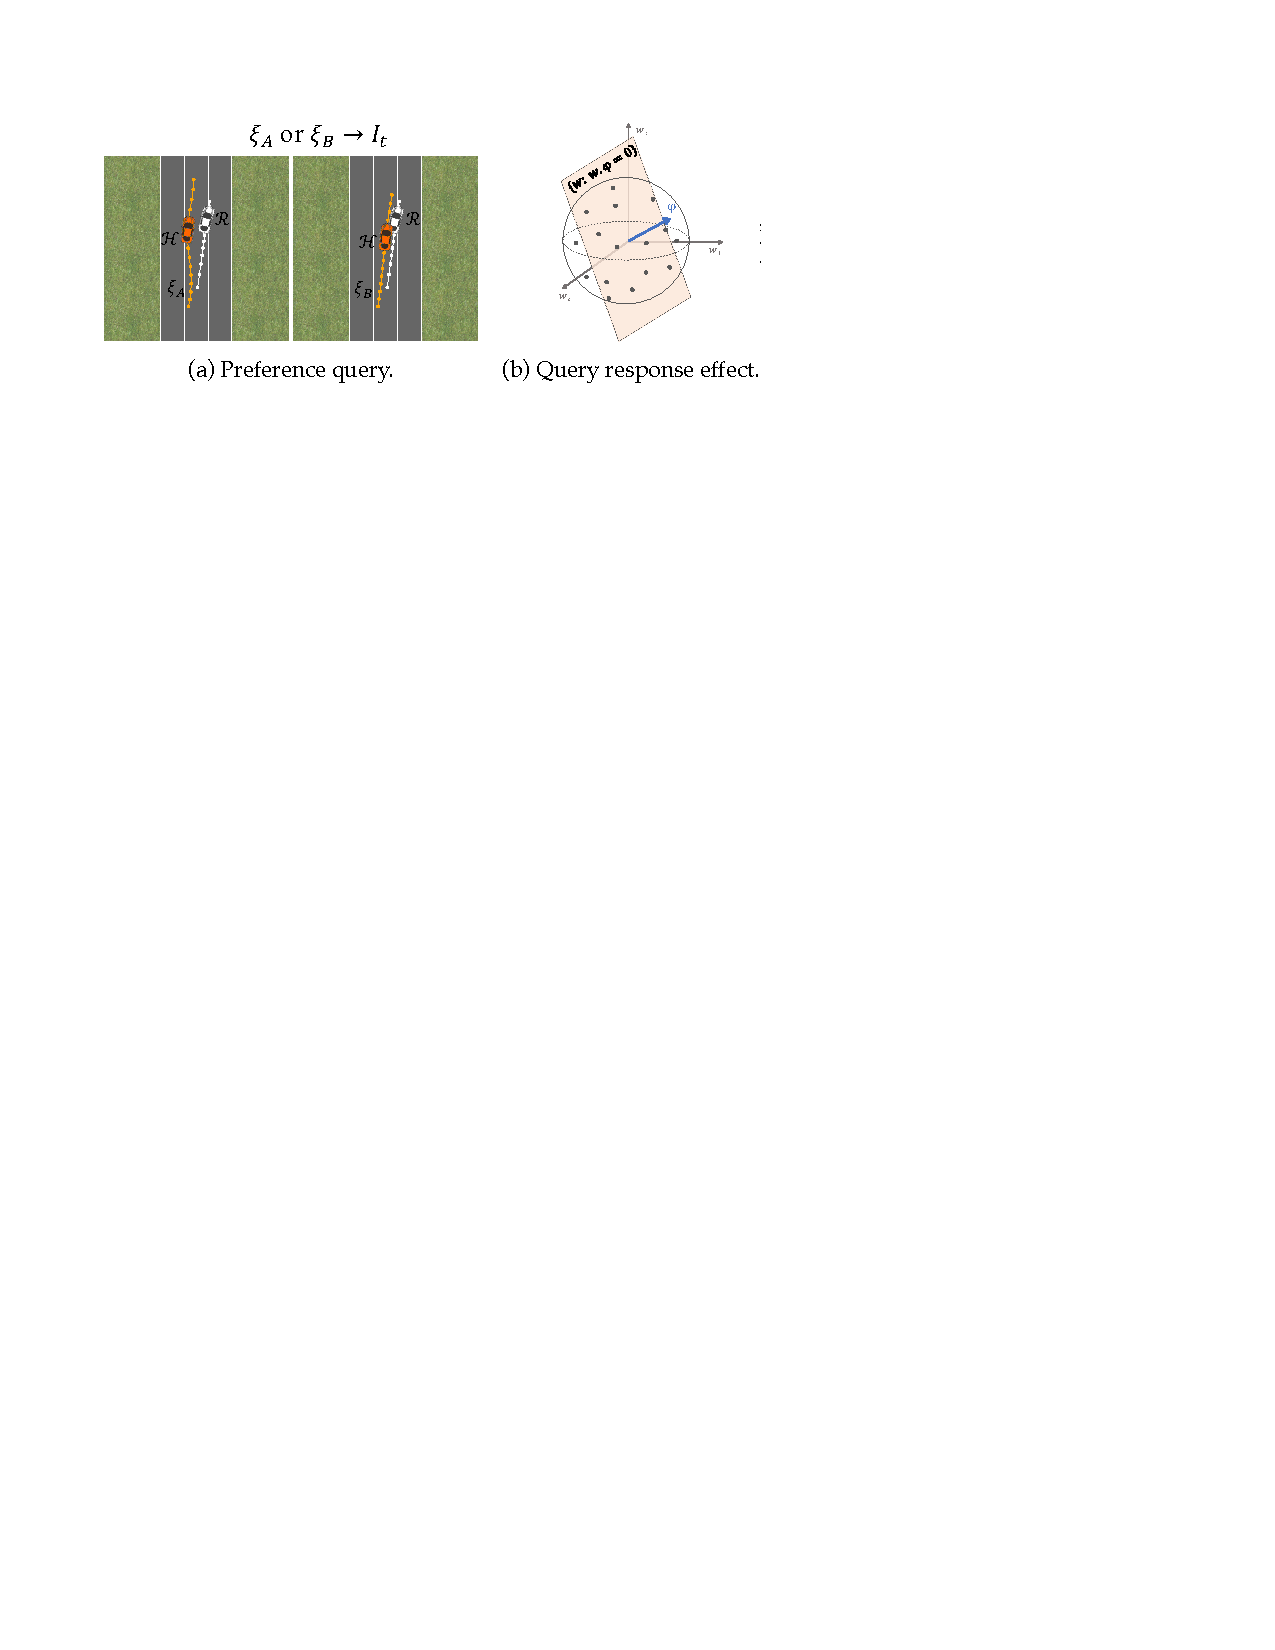
\includegraphics[width = 0.8\textwidth]{./Query}
  	\vspace{0.25cm}
  	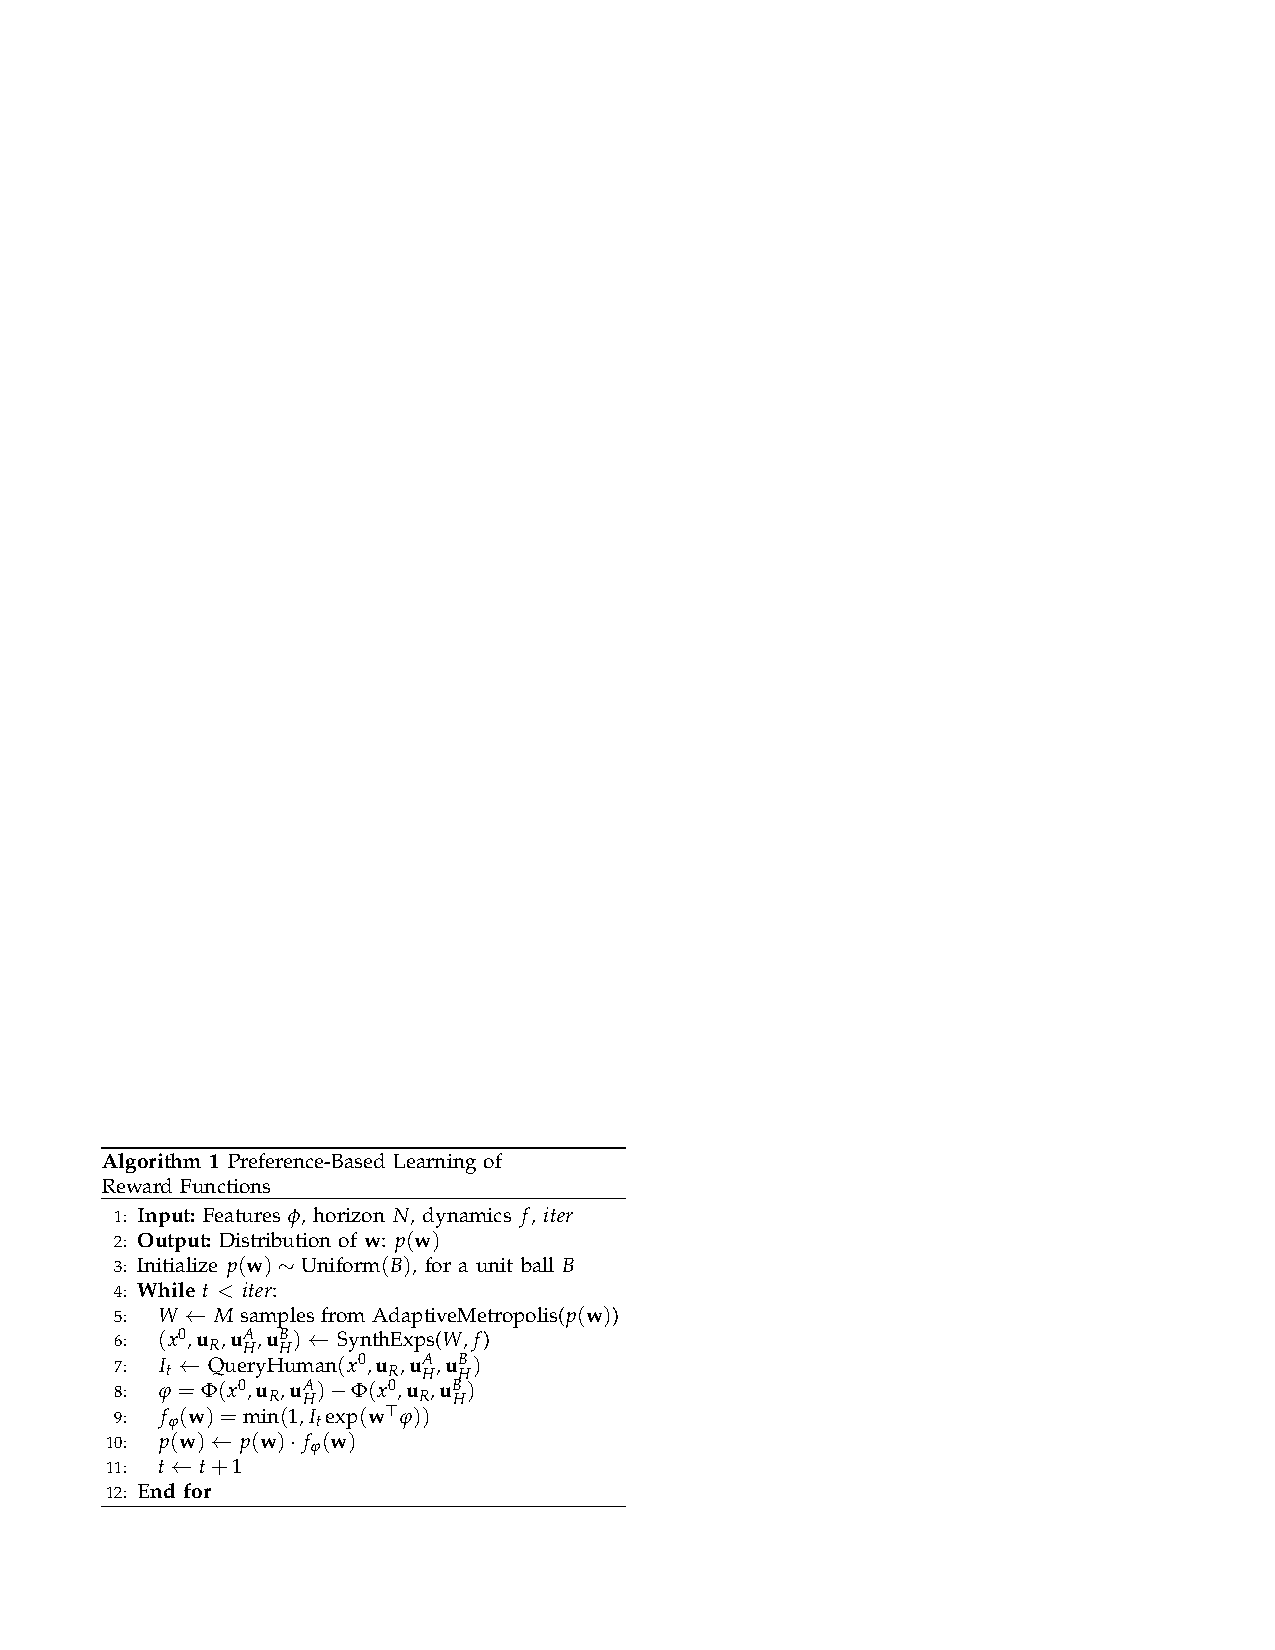
\includegraphics[width = 0.45\textwidth]{./Algo}
  	\end{center}
  	% \includegraphics[width = 0.5\textwidth,right]{./QueryResponse}

  	%   	\begin{figure}

  	% \end{figure}
%   	\hfill
%   	\begin{figure}
%   	  	  	\includegraphics[width = 0.4\textwidth]{./PrefQuery}
%   	\includegraphics[width = 0.5\textwidth]{./QueryResponse}
% \end{figure}
\end{frame}

\begin{frame}[t]{Results}
	\begin{center}
  	\includegraphics[width = 0.9\textwidth]{./BigResult}
  	\end{center}
  	\begin{center}
  	% \vspace{0.25cm}
  	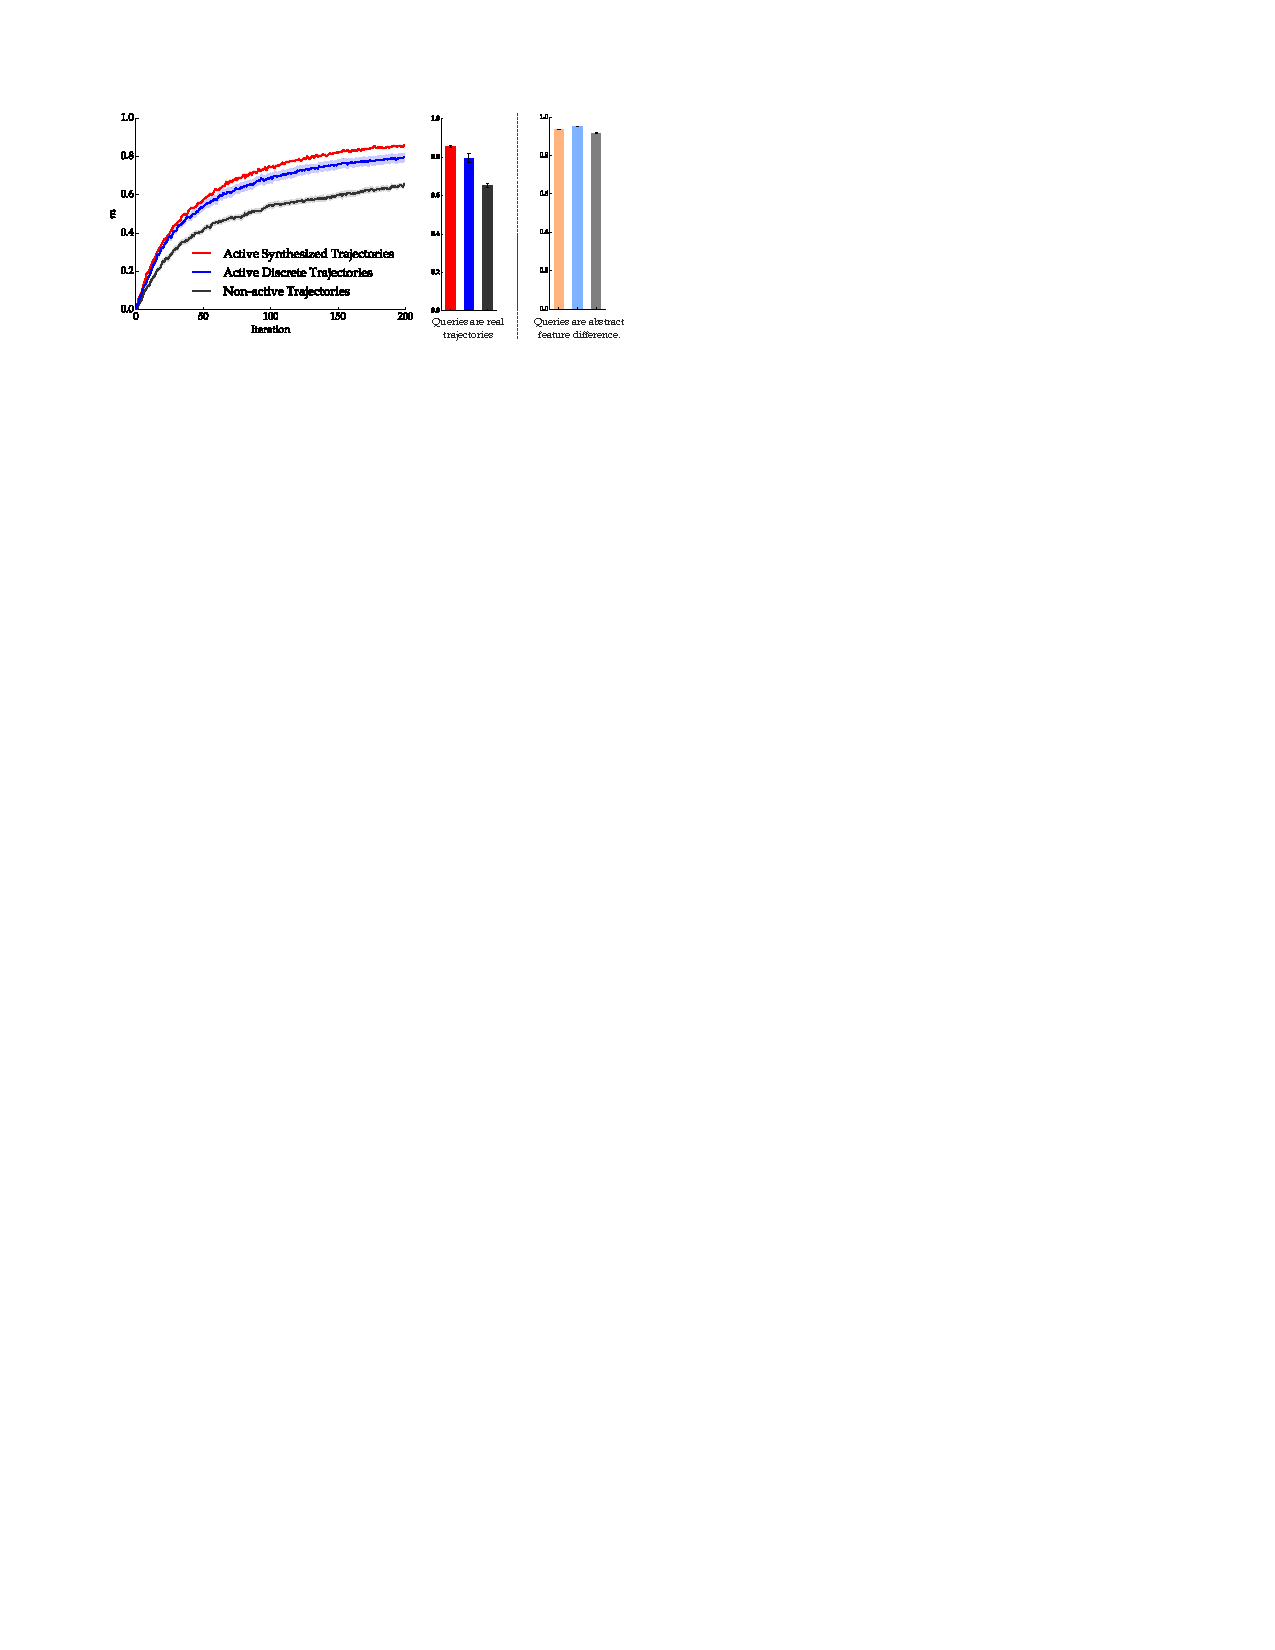
\includegraphics[width = 0.55\textwidth]{./SmallResult}
  	\end{center}
\end{frame}

\begin{frame}[t]{Discussion}
\begin{itemize} \itemsep 0.05in
	\item What is novel/interesting?
	\begin{itemize} \itemsep 0.025in
		\item \textbf{preference-based} approach allows users to compare two trajectories in various scenarios without having to demonstrate a full trajectory (of how they would like to drive, not how they actually drive)
		\item \textbf{active} enables choosing informative test cases otherwise difficult to encounter in driving scenarios; addresses the limitation of training data sparsity/informativeness
		\item In-depth investigation of the effect of \textbf{synthesis} of real trajectories for dynamical systems compared to relying on a discrete set
	\end{itemize}
	\item Limitations
	\begin{itemize} \itemsep 0.025in
		\item Markov assumption is inherently built into system dynamics
		\item Feature selection is not active/based on expert knowledge
		\item Reward function is constrained to be linear in the feature space
		\item The entire formulation is for a human $H$ with only one other robot $R$
		\item Formulation of $\textbf{w}_{true}$ was unclear
		\item Experiments:
		\begin{itemize} \itemsep 0.025in
			\item potential functions' based reward function
			\item $f_{HR}$ assumed as a simple point mass-dynamics model
		\end{itemize}
	\end{itemize}
\end{itemize}
\end{frame}

\begin{frame}[t]{Questions}
	\begin{center} \Huge Questions? \end{center}
\end{frame}

% Save final frame number, so that backup slides are not counted
\newcounter{finalframe}
\setcounter{finalframe}{\value{framenumber}}

% \begin{frame}[t]{Backup Slide 1}
% 	\begin{itemize} %\itemsep 0.1in
% 		\item Blah blah blah ...
% 	\end{itemize}
% \end{frame}

\begin{frame}[allowframebreaks]{References}
	\tiny
	\def\newblock{}
	\bibliography{IEEEabrv,ref}		% specify bibliography file
									% (ref.bib) here
\end{frame}

\setcounter{framenumber}{\value{finalframe}}
% Set up so that backup slides are not counted in total slides

\end{document}
